\documentclass[hidelinks,12pt,a4paper]{article}
\usepackage[italian]{babel}
\usepackage[utf8]{inputenc}
\usepackage{fourier} 

% Images
\usepackage{graphicx}
\usepackage{caption}
\usepackage{subcaption}
\usepackage{float}
\graphicspath{ {../Images} }

% Stop hyphenation
\usepackage[none]{hyphenat}

% Adjust paragraph.
\usepackage{changepage}

% Write over image.
\usepackage{tikz}

% Adjust image dim.
\usepackage{adjustbox}

% License
\usepackage[
type={CC},
modifier={by-nc-sa},
version={4.0},
]{doclicense}

\begin{document}
	
	\title{\textbf{\centering{Laboratorio creativo per bambini}\\Trova le opere dentro il museo.}}
	\author{Alice Balestieri}
	\date{}
	
	\maketitle
	\newpage
	
	\tableofcontents
	\newpage
	
	\section{Come giocare}
	\begin{center}
		\textbf{Le regole sono rivolte agli operatori.}
	\end{center}
	
	\subsection{Variante 1}
	Dopo aver ritagliato le immagini, consegnarle a rotazione ai bambini fino ad esaurire il mazzo, aggiungendo qualora ne fossero sprovvisti, delle penne con le quali poter scrivere sulla carta.\\
	A partire dal suggerimento fornito dalla porzione d'immagine che compone la carta, i bambini dovranno girare liberamente nel museo per ritrovare l'opera, e ricopiare la descrizione della suddetta nel riquadro posto sotto la porzione d'immagine.\\
	Quando tutti i bambini hanno finito di completare il compito, procedere con la correzione spiegata, concentrandosi in caso di errore sulle differenze tra l'opera da individuare e quella riportata dal bambino.
	
	\subsection{Variante 2}
	Dopo aver ritagliato le immagini, consegnarle a rotazione ai bambini fino ad esaurire il mazzo, aggiungendo qualora ne fossero sprovvisti, delle penne con le quali poter scrivere sulla carta.\\
	A partire dal suggerimento fornito dalla porzione d'immagine che compone la carta, i bambini dovranno esercitare la propria memoria cercando d'individuare l'opera a partire dal suggerimento e scrivendo nel riquadro sottostante quante più informazioni possibili sull'opera.\\
	Far scrivere a tutti i bambini i loro nomi su una estremità della carte possedute e successivamente raccogliere tutte le carte per procedere con la correzione spiegata.\\
	 Muovendosi nel museo, raggiungere assieme i bambini la posizione delle varie opere, e per ogni opera, raggruppare i bambini che hanno dovuto descriverla (i loro nomi sono scritti sulle carte), leggere quello che hanno scritto, per poi fare il confronto con la suddetta.
	
	
	\vspace*{\fill}
	\centering
	\fboxrule=2pt
	\fbox
	{
		\begin{minipage}{\linewidth}
			In caso di dubbi per la correzione, tenere una copia digitale di questo documento consultabile dallo "smartphone". Nella sezione "Immagini e didascalie" ogni immagine frammentata è presentata con la relativa didascalia posta inferiormente.
		\end{minipage}
	}

	\newpage
	\section{Gestione immagini nel documento}
	
	\begin{tikzpicture}
		\node[anchor=south west,inner sep=0] (image) at (0,0) {\includegraphics[scale=0.85]{example-image}};
		\begin{scope}[x={(image.south east)},y={(image.north west)}]
			\draw[help lines,xstep=.1,ystep=.1] (0,0) grid (1,1);
			\foreach \x in {0,1,...,9} { \node [anchor=north] at (\x/10,0) {0.\x}; }
			\foreach \y in {0,1,...,9} { \node [anchor=east] at (0,\y/10) {0.\y}; }
		\end{scope}
	\end{tikzpicture}

	\newpage
	\section{Immagini e didascalie}
	
	%---------- Begin page ----------
	\begin{adjustwidth}{-30mm}{-30mm}
		% Rule [trim={left bottom right top},clip]
		
		% Superior section
		\begin{minipage}{\linewidth}
			\fbox{
				\begin{minipage} [l] [\dimexpr 0.430\textwidth \relax] [t] {\dimexpr .460\textwidth \relax}
					\medskip
					\centering
					\begin{tikzpicture}
						\node[anchor=south west,inner sep=0] (image) at (0,0) {\includegraphics[]{Mengaroni_Ferruccio-Medusa.jpg}};
						\begin{scope}[x={(image.south east)},y={(image.north west)}]
							\draw[draw=none,fill=white] (0,0.5) rectangle (0.25,1);
						\end{scope}
					\end{tikzpicture}
					
					\vspace*{\fill}
					\fboxrule=4pt{
					\framebox[\textwidth]{\rule{0pt}{55pt}}}
					
				\end{minipage}
		}%
			\hfill{
				\fbox{
					\begin{minipage} [r] [\dimexpr 0.430\textwidth \relax] [t] {\dimexpr .460\textwidth \relax}
						\medskip
						\centering
						\adjustbox{trim={0.5\width}  {0.5\height} 0 0,clip}%
						{\includegraphics[scale=2]{Mengaroni_Ferruccio-Medusa.jpg}}
						
						\vspace*{\fill}
						\fboxrule=4pt{
							\framebox[\textwidth]{\rule{0pt}{55pt}}}
					\end{minipage}
				}
			}
		\end{minipage}
	
	\vspace{4mm}
	
	%--- Bottom section
		\begin{minipage}{\linewidth}
		\fbox{
			\begin{minipage} [l] [\dimexpr 0.430\textwidth \relax] [t] {\dimexpr .460\textwidth \relax}
				\medskip
				\centering
				\adjustbox{trim=0 0 {0.5\width} {0.5\height},clip}%
				{\includegraphics[scale=2]{Mengaroni_Ferruccio-Medusa.jpg}}
				
				\vspace*{\fill}
				\fboxrule=4pt{
				\framebox[\textwidth]{\rule{0pt}{55pt}}}
			\end{minipage}
		}%
		%
		\hfill{
			\fbox{
				\begin{minipage} [r] [\dimexpr 0.430\textwidth \relax] [t] {\dimexpr .460\textwidth \relax}
					\medskip
					\centering
					\adjustbox{trim={0.5\width} 0 0 {0.5\height},clip}%
					{\includegraphics[scale=2]{Mengaroni_Ferruccio-Medusa.jpg}}
					
					\vspace*{\fill}
					\fboxrule=4pt{
						\framebox[\textwidth]{\rule{0pt}{55pt}}}
				\end{minipage}
			}
		}
	\end{minipage}
	\end{adjustwidth}

	
	\vspace*{\fill}
	\centering
	\fboxrule=2pt{
	\fbox
	{
		\begin{minipage}{\linewidth}
			\centering
		Mengaroni Ferruccio - Medusa.
		\end{minipage}
	}}
	%---------- End page ----------
	
	%---------- Begin page ----------
	\begin{adjustwidth}{-30mm}{-30mm}
		
		% Superior section
		\begin{minipage}{\linewidth}
			\fbox{
				\begin{minipage} [l] [\dimexpr 0.430\textwidth \relax] [t] {\dimexpr .460\textwidth \relax}
					\medskip
					\centering
					\adjustbox{trim=0 {0.5\height} {0.5\width} 0,clip}%
					{\includegraphics[scale=0.095]{Bellini_Giovanni-Incoronazione_della_Vergine.jpg}}
					
					\vspace*{\fill}
					\fboxrule=4pt{
						\framebox[\textwidth]{\rule{0pt}{55pt}}}
					
				\end{minipage}
			}%
			\hfill{
				\fbox{
					\begin{minipage} [r] [\dimexpr 0.430\textwidth \relax] [t] {\dimexpr .460\textwidth \relax}
						\medskip
						\centering
						\adjustbox{trim={0.5\width}  {0.5\height} 0 0,clip}%
						{\includegraphics[scale=0.095]{Bellini_Giovanni-Incoronazione_della_Vergine.jpg}}
						
						\vspace*{\fill}
						\fboxrule=4pt{
							\framebox[\textwidth]{\rule{0pt}{55pt}}}
					\end{minipage}
				}
			}
		\end{minipage}
		
		\vspace{4mm}
		
		%--- Bottom section
		\begin{minipage}{\linewidth}
			\fbox{
				\begin{minipage} [l] [\dimexpr 0.430\textwidth \relax] [t] {\dimexpr .460\textwidth \relax}
					\medskip
					\centering
					\adjustbox{trim=0 0 {0.5\width} {0.5\height},clip}%
					{\includegraphics[scale=0.095]{Bellini_Giovanni-Incoronazione_della_Vergine.jpg}}
					
					\vspace*{\fill}
					\fboxrule=4pt{
						\framebox[\textwidth]{\rule{0pt}{55pt}}}
				\end{minipage}
			}%
			%
			\hfill{
				\fbox{
					\begin{minipage} [r] [\dimexpr 0.430\textwidth \relax] [t] {\dimexpr .460\textwidth \relax}
						\medskip
						\centering
						\adjustbox{trim={0.5\width} 0 0 {0.5\height},clip}%
						{\includegraphics[scale=0.095]{Bellini_Giovanni-Incoronazione_della_Vergine.jpg}}
						
						\vspace*{\fill}
						\fboxrule=4pt{
							\framebox[\textwidth]{\rule{0pt}{55pt}}}
					\end{minipage}
				}
			}
		\end{minipage}
	\end{adjustwidth}
	
	
	\vspace*{\fill}
	\centering
	\fboxrule=2pt{
		\fbox
		{
			\begin{minipage}{\linewidth}
				\centering
				Bellini Giovanni - Incoronazione della Vergine.
			\end{minipage}
	}}
	%---------- End page ----------
	
	%---------- Begin page ----------
	\begin{adjustwidth}{-30mm}{-30mm}
		
		% Superior section
		\begin{minipage}{\linewidth}
			\fbox{
				\begin{minipage} [l] [\dimexpr 0.430\textwidth \relax] [t] {\dimexpr .460\textwidth \relax}
					\medskip
					\centering
					\adjustbox{trim=0 {0.5\height} {0.5\width} 0,clip}%
					{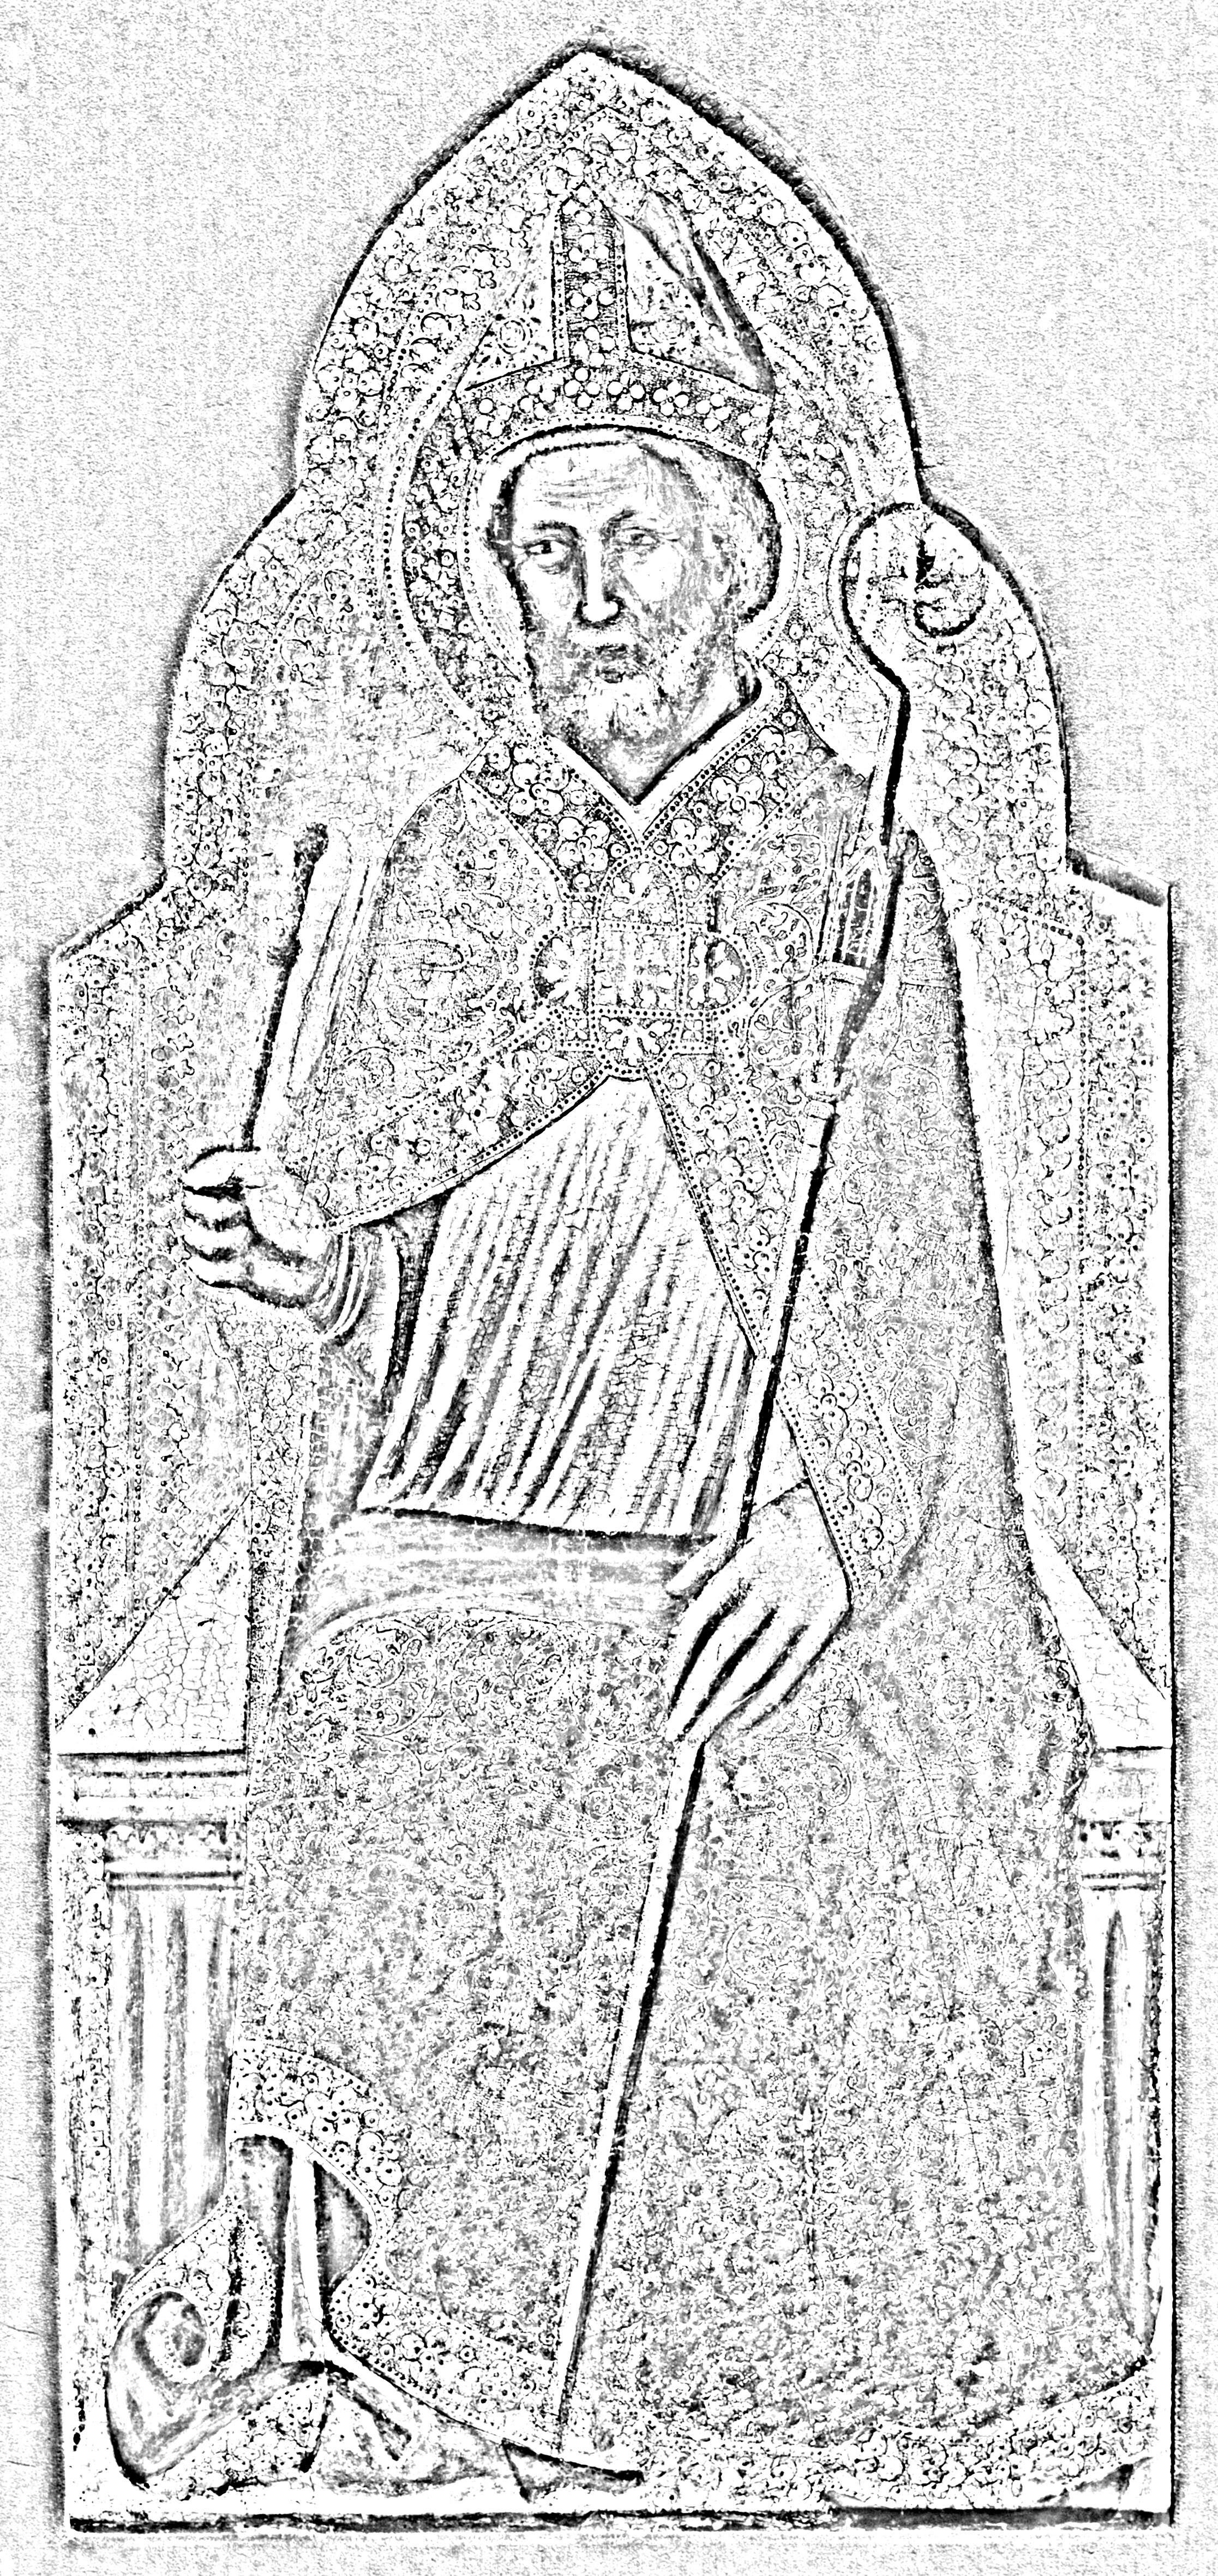
\includegraphics[scale=0.068]{Vitale_da_Bologna-Santo_Ambrogio_in_trono.jpg}}
					
					\vspace*{\fill}
					\fboxrule=4pt{
						\framebox[\textwidth]{\rule{0pt}{55pt}}}
					
				\end{minipage}
			}%
			\hfill{
				\fbox{
					\begin{minipage} [r] [\dimexpr 0.430\textwidth \relax] [t] {\dimexpr .460\textwidth \relax}
						\medskip
						\centering
						\adjustbox{trim={0.5\width}  {0.5\height} 0 0,clip}%
						{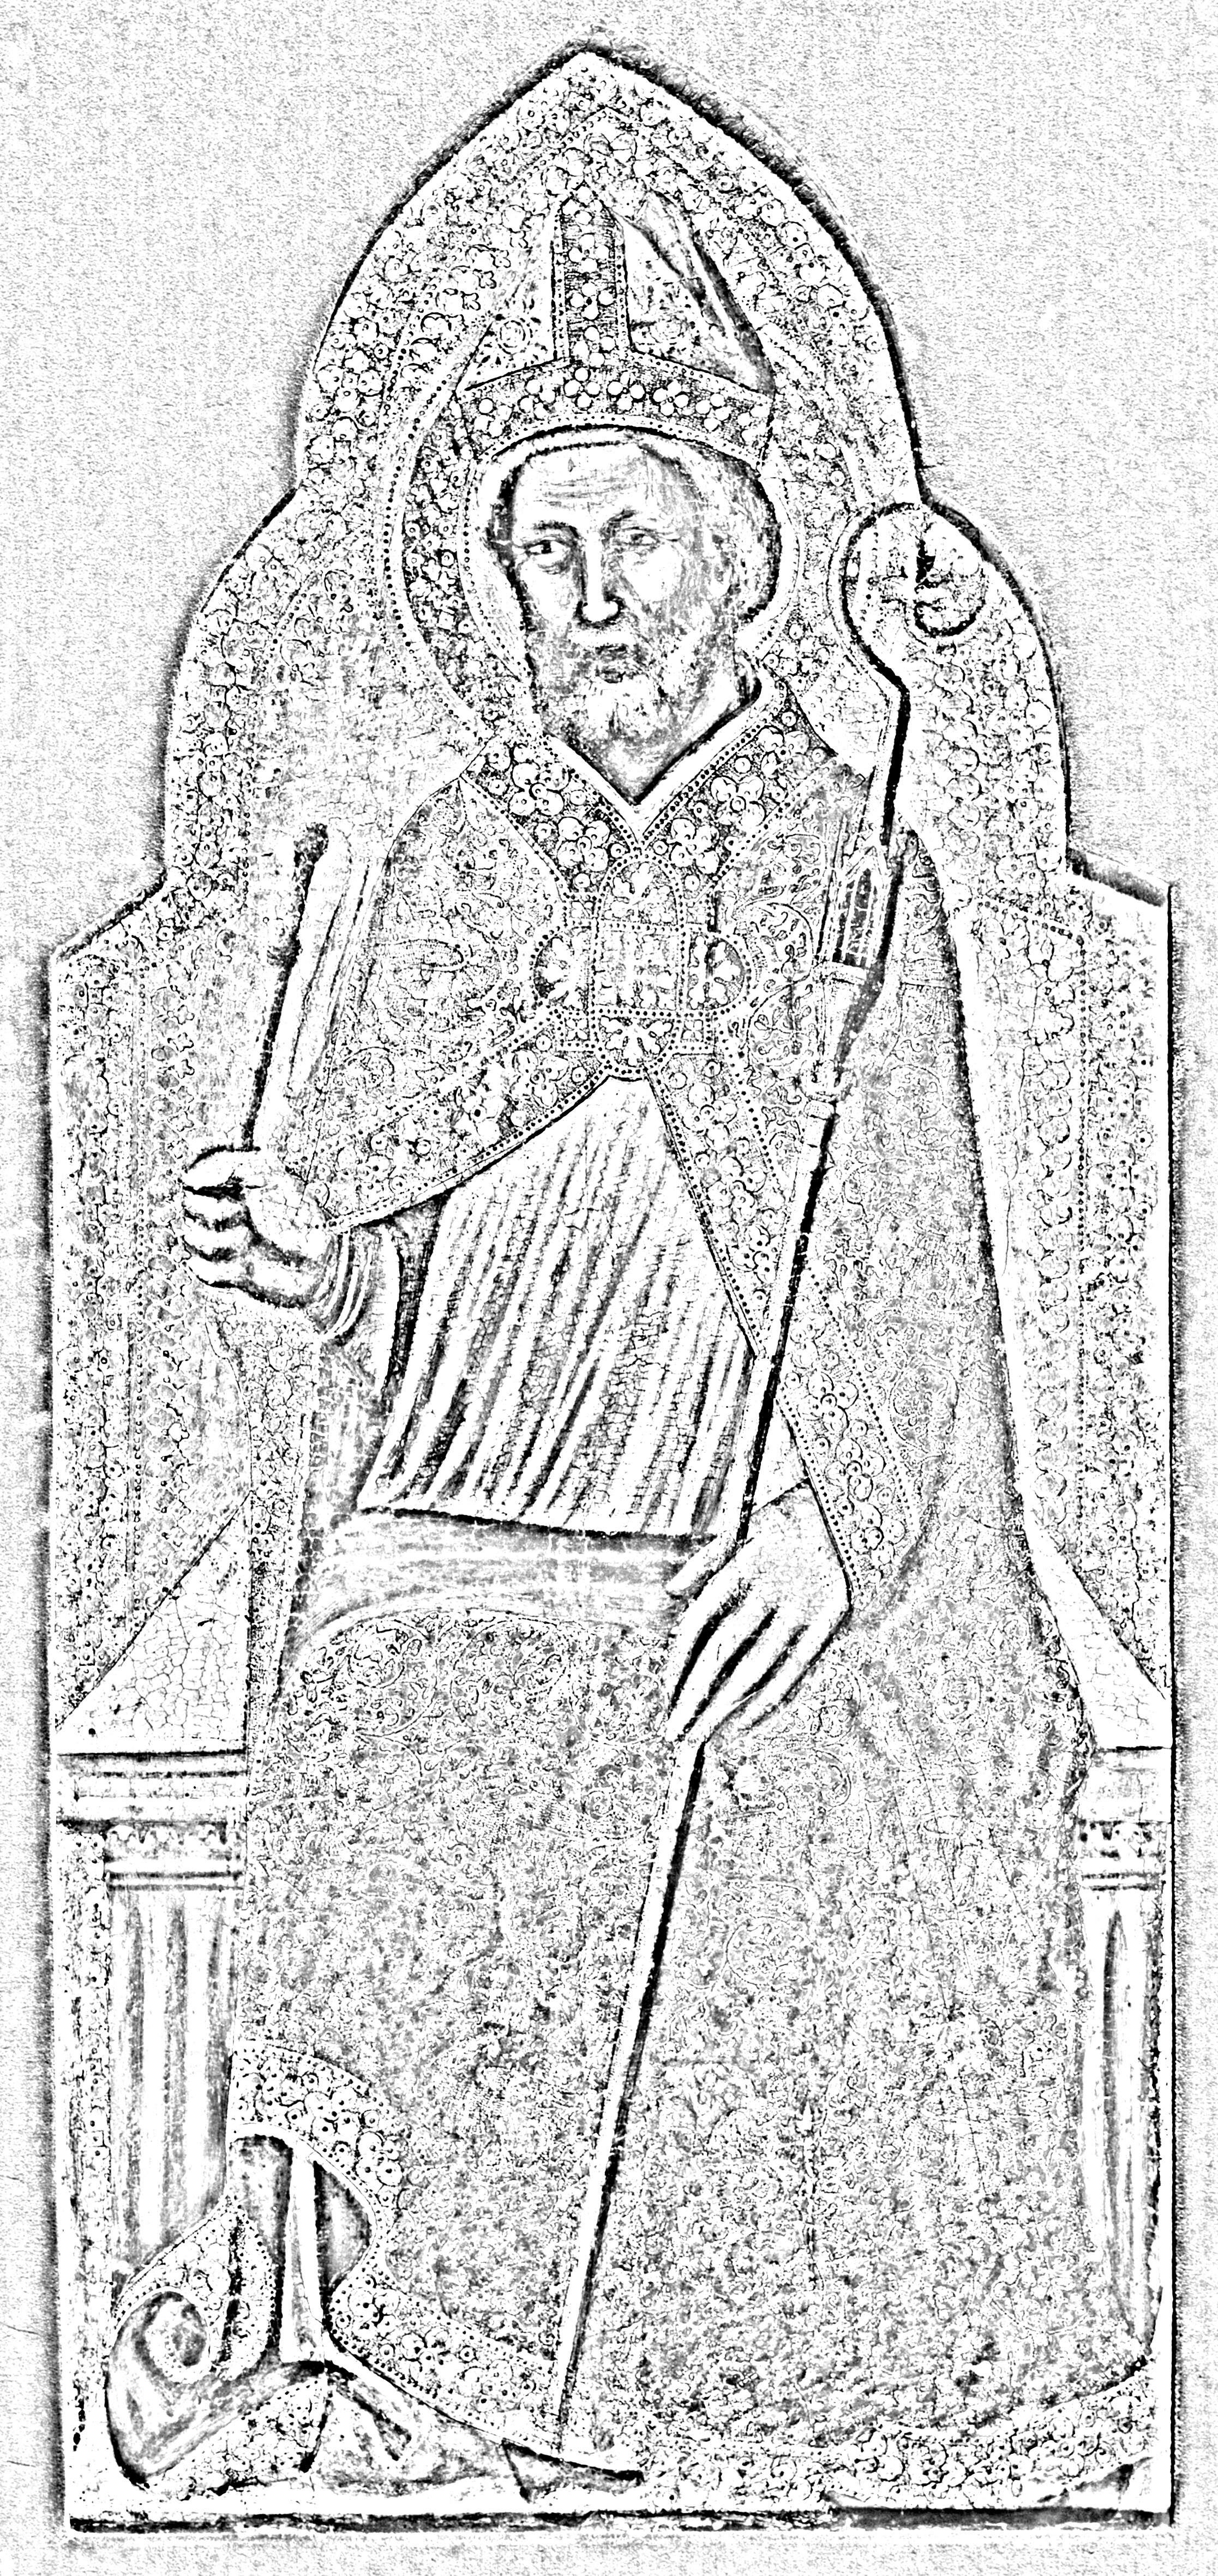
\includegraphics[scale=0.068]{Vitale_da_Bologna-Santo_Ambrogio_in_trono.jpg}}
						
						\vspace*{\fill}
						\fboxrule=4pt{
							\framebox[\textwidth]{\rule{0pt}{55pt}}}
					\end{minipage}
				}
			}
		\end{minipage}
		
		\vspace{4mm}
		
		%--- Bottom section
		\begin{minipage}{\linewidth}
			\fbox{
				\begin{minipage} [l] [\dimexpr 0.430\textwidth \relax] [t] {\dimexpr .460\textwidth \relax}
					\medskip
					\centering
					\adjustbox{trim=0 0 {0.5\width} {0.5\height},clip}%
					{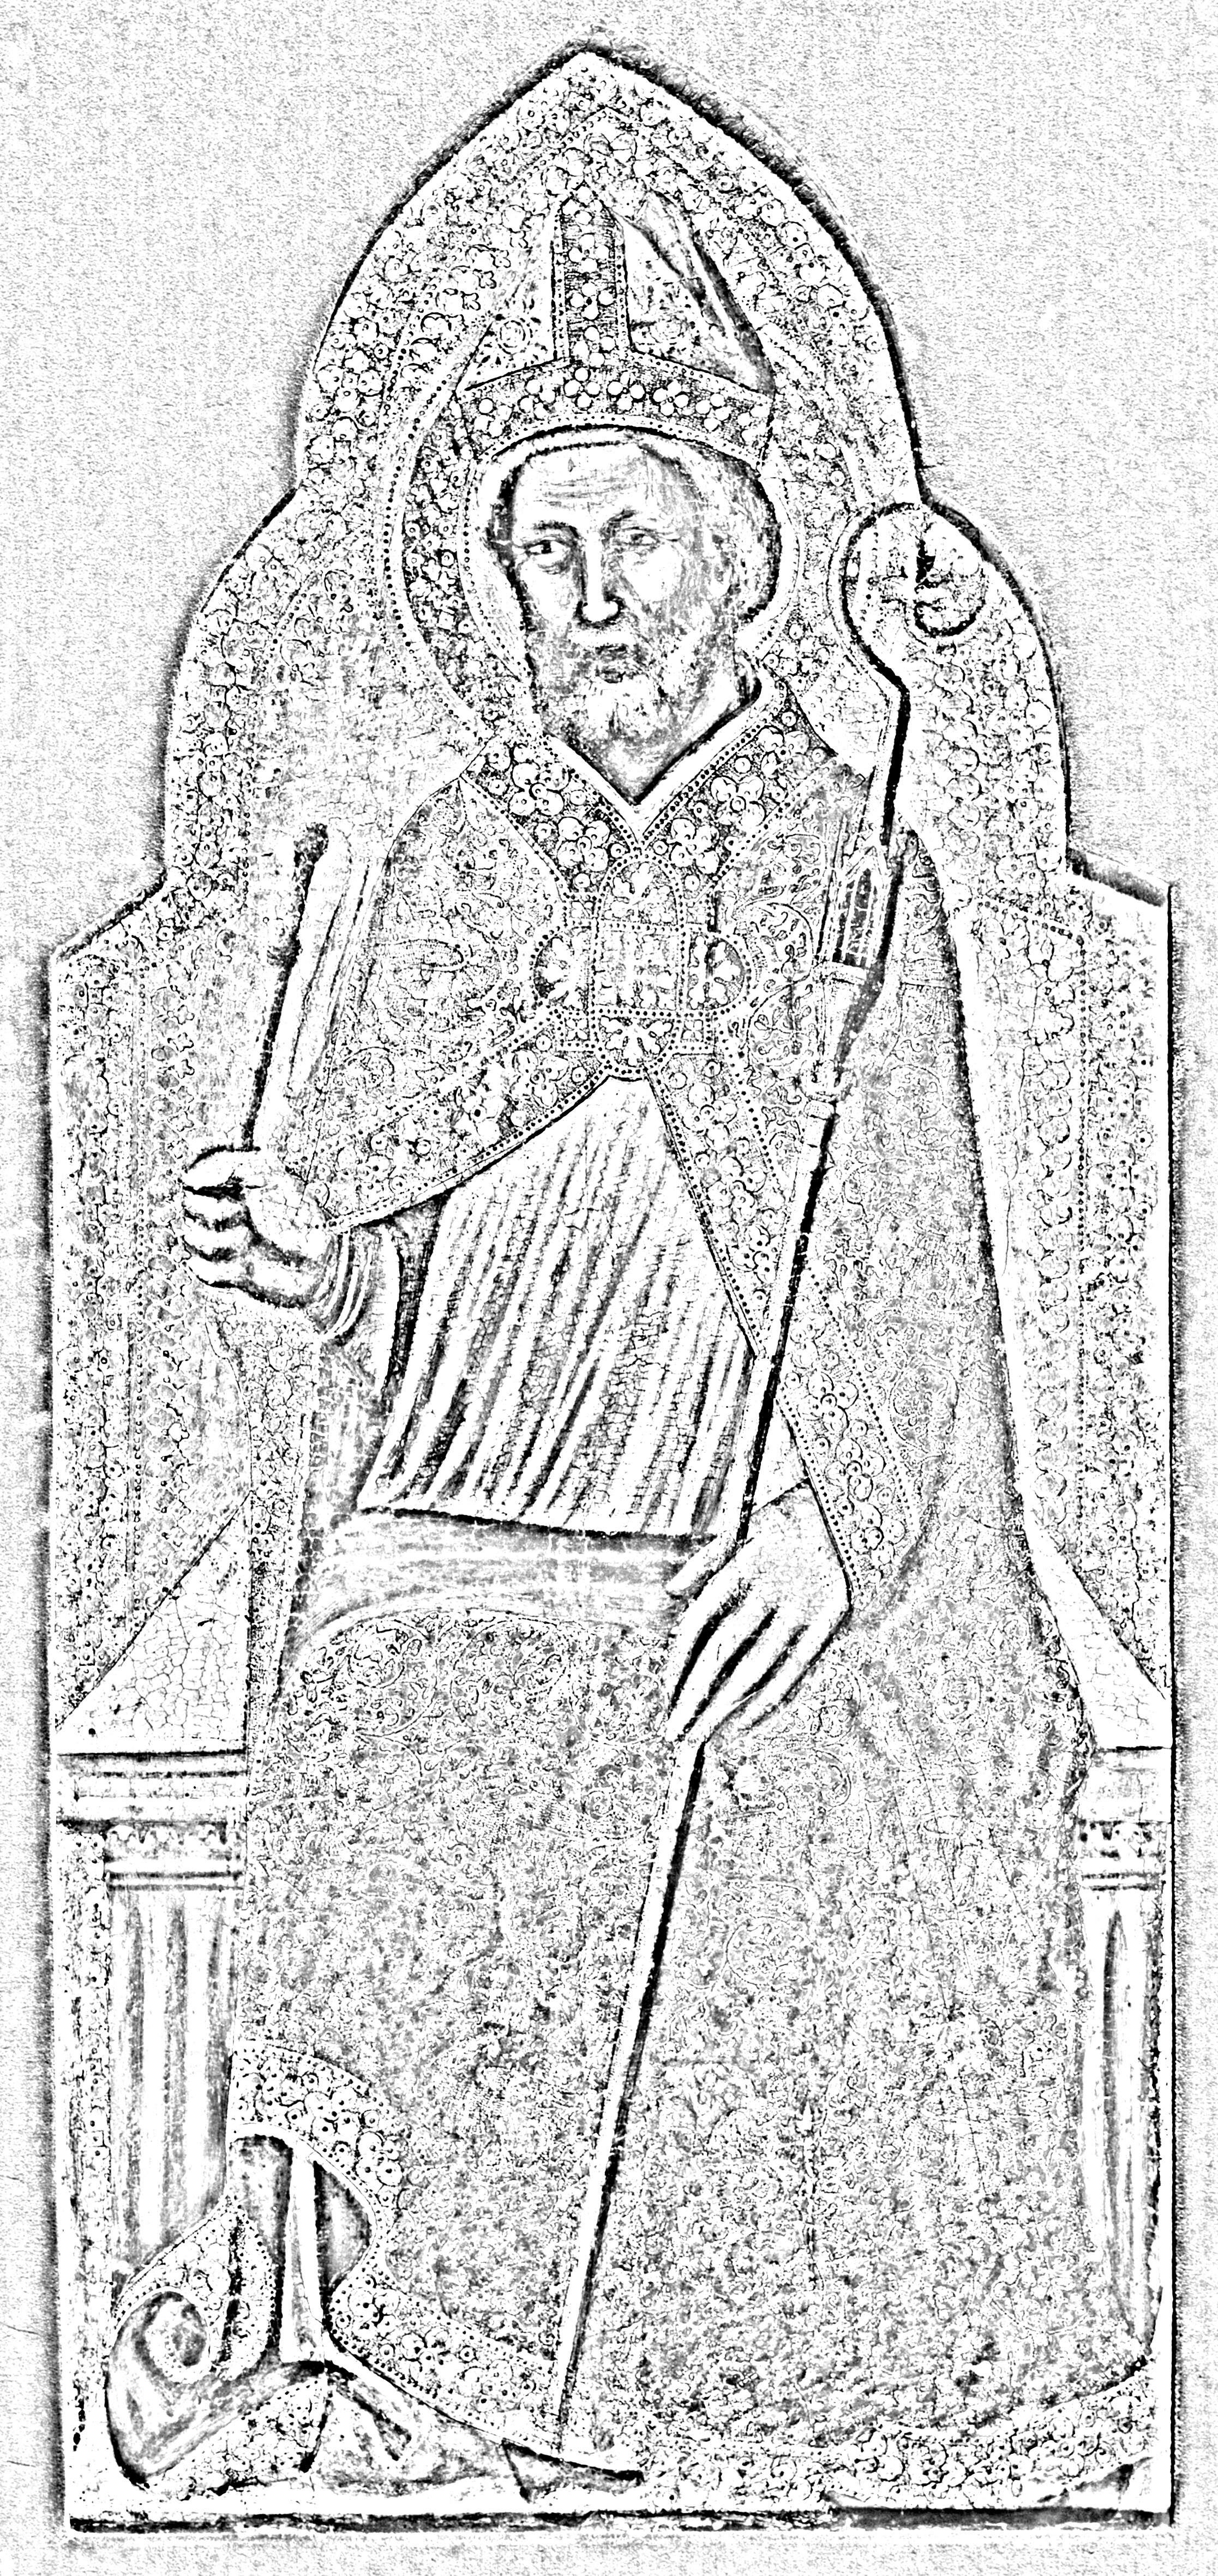
\includegraphics[scale=0.068]{Vitale_da_Bologna-Santo_Ambrogio_in_trono.jpg}}
					
					\vspace*{\fill}
					\fboxrule=4pt{
						\framebox[\textwidth]{\rule{0pt}{55pt}}}
				\end{minipage}
			}%
			%
			\hfill{
				\fbox{
					\begin{minipage} [r] [\dimexpr 0.430\textwidth \relax] [t] {\dimexpr .460\textwidth \relax}
						\medskip
						\centering
						\adjustbox{trim={0.5\width} 0 0 {0.5\height},clip}%
						{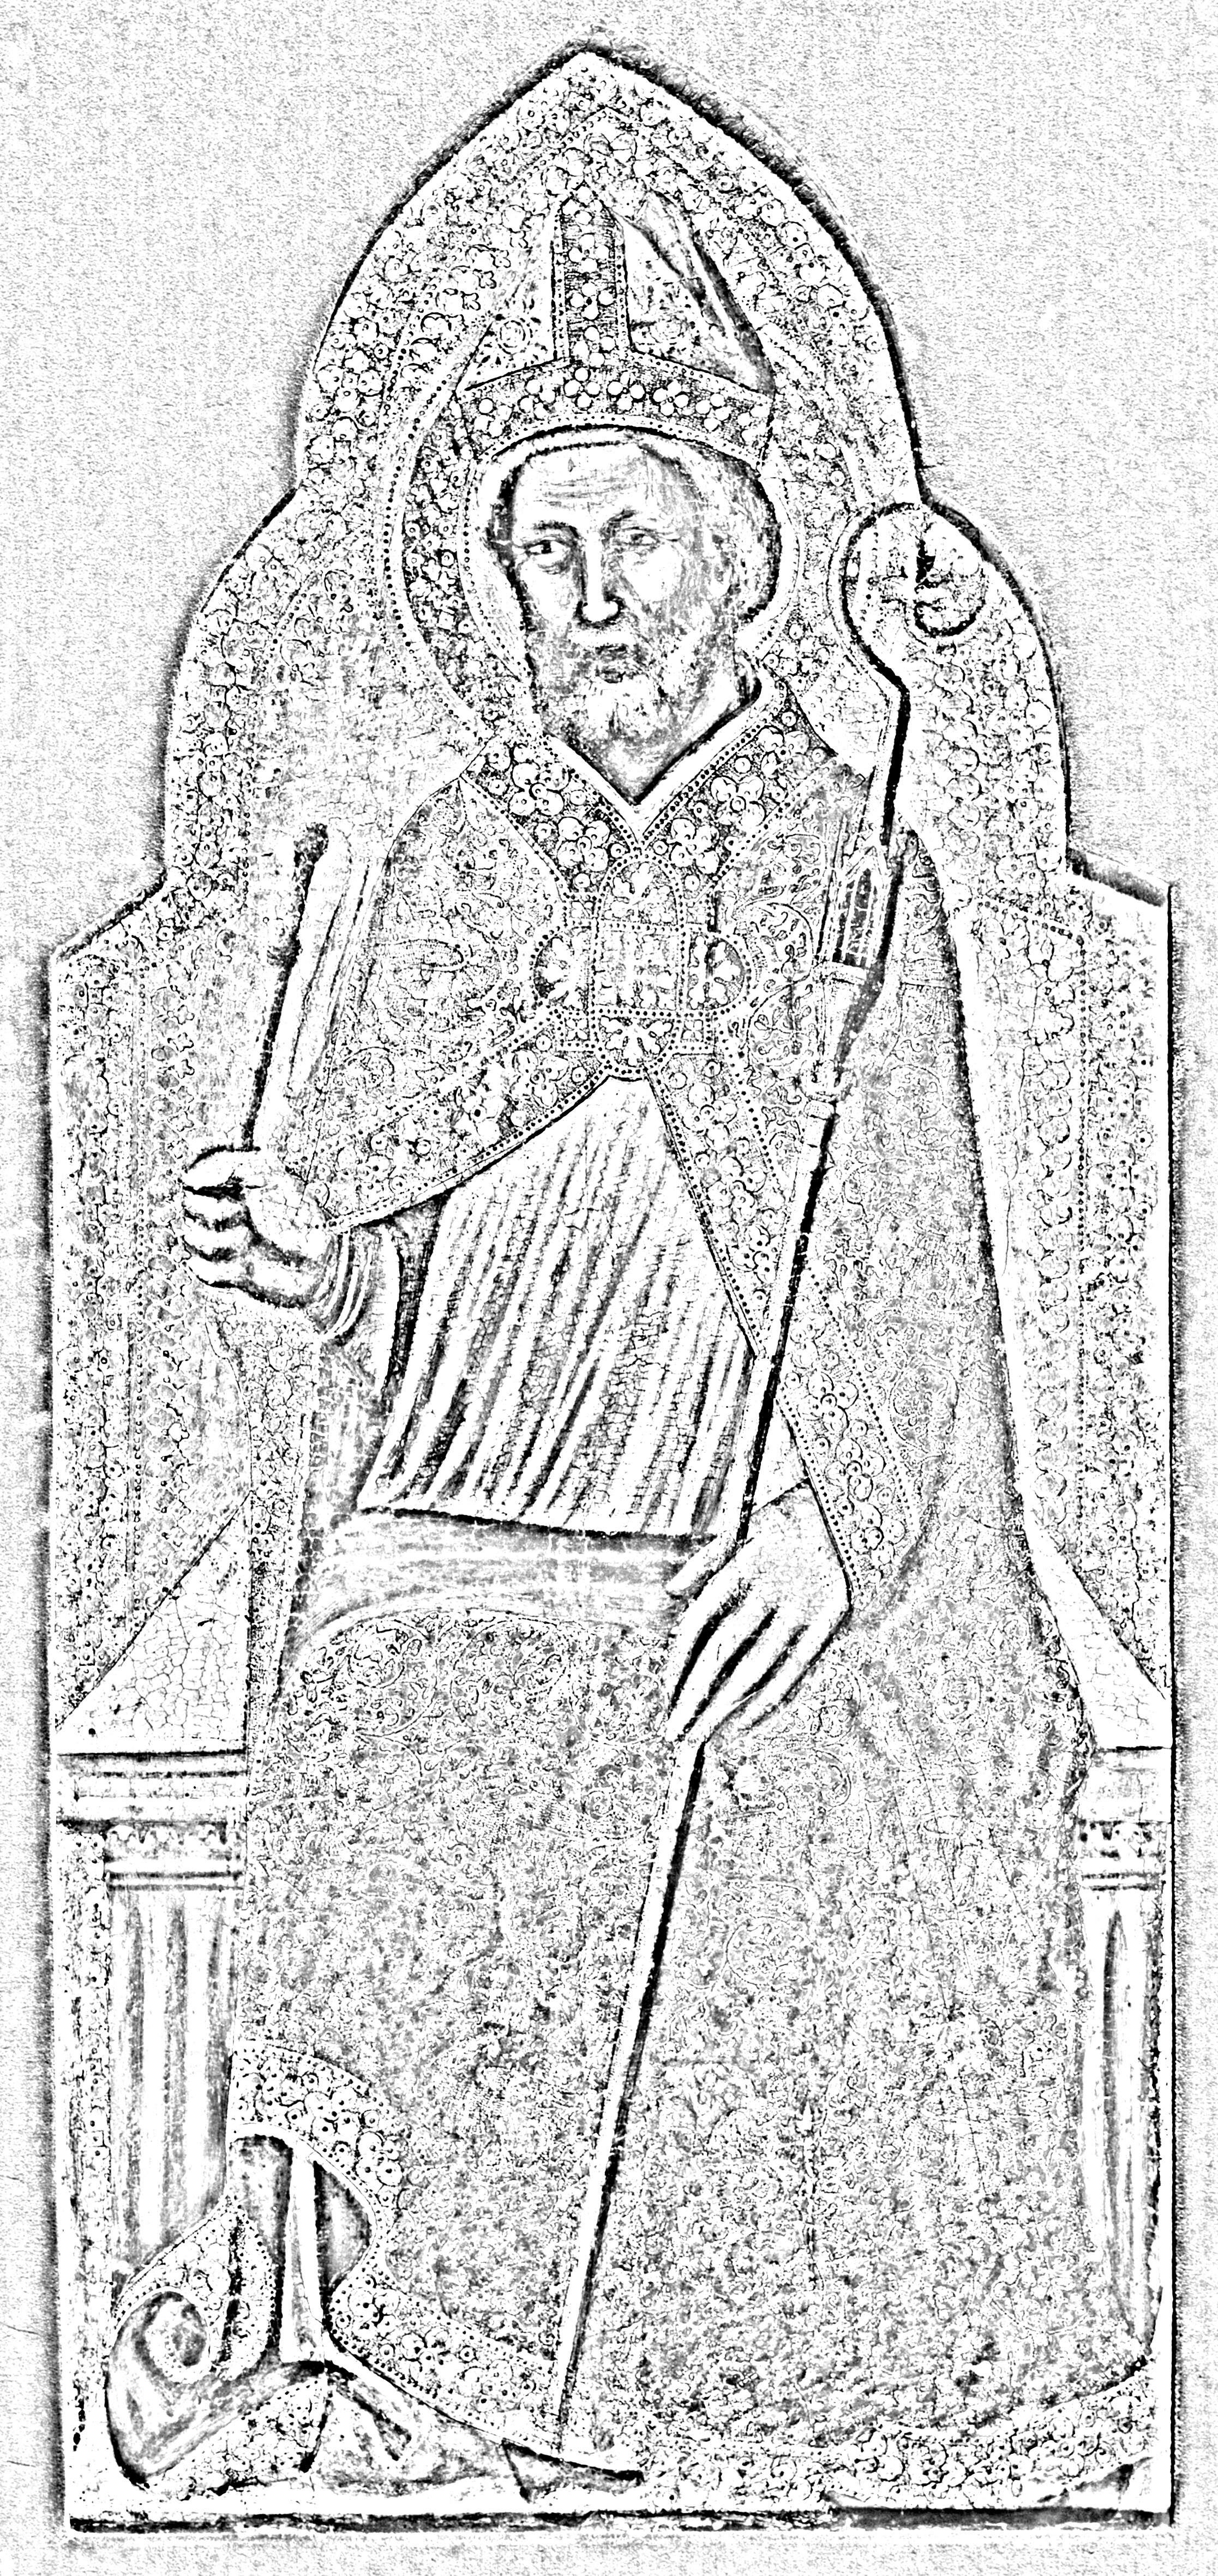
\includegraphics[scale=0.068]{Vitale_da_Bologna-Santo_Ambrogio_in_trono.jpg}}
						
						\vspace*{\fill}
						\fboxrule=4pt{
							\framebox[\textwidth]{\rule{0pt}{55pt}}}
					\end{minipage}
				}
			}
		\end{minipage}
	\end{adjustwidth}
	
	
	\vspace*{\fill}
	\centering
	\fboxrule=2pt{
		\fbox
		{
			\begin{minipage}{\linewidth}
				\centering
				Vitale da Bologna - Santo Ambrogio in trono.
			\end{minipage}
	}}
	%---------- End page ----------
\end{document}	